%!BIB program = bibtex
\documentclass[9pt, twocolumn, twoside, lineno]{pnas-new}
% Use the lineno option to display guide line numbers if required.

% PNAS研究论文模板
\templatetype{pnasresearcharticle} % Choose template 
% {pnasresearcharticle} = Template for a two-column research article
% {pnasmathematics} %= Template for a one-column mathematics article
% {pnasinvited} %= Template for a PNAS invited submission
% \usepackage{cite}
	
% 文章标题:“流域尺度的水资源利用体系:过渡框架和发展困局”
\title{Water resource utilization regimes at a basin scale: transition framework and development traps}

% Use letters for affiliations, numbers to show equal authorship (if applicable) and to indicate the corresponding author
% 作者列表
\author[a, b]{Shuang Song}  % 宋爽,一作
\author[a, b, 1]{Shuai Wang}  % 王老师,通讯
\author[a, b]{Bojie Fu}  % 傅老师
\author[c, d]{Xutong Wu}  % 武旭同

% 机构列表
\affil[a]{ % 北师大地表国重
	State Key Laboratory of Earth Surface Processes and Resource Ecology, 
	Faculty of Geographical Science, 
	Beijing Normal University, 
	Beijing 100875, 
	P.R. China
}
\affil[b]{ % 北师大地理学部
	Institute of Land Surface System and Sustainability, 
	Faculty of Geographical Science, 
	Beijing Normal University, 
	Beijing 100875, 
	P.R. China
}
\affil[c]{ % 北大城环
	College of Urban and Environmental Sciences, 
	Peking University, 
	Beijing 100871, 
	P.R. China
}
\affil[d]{ % 中科院生态中心
	State Key Laboratory of Urban and Regional Ecology, 
	Research Center for Eco-Environmental Sciences, 
	Chinese Academy of Sciences, 
	Beijing 100085, 
	P.R. China 
}

% Please give the surname of the lead author for the running footer
% 领衔作者
\leadauthor{Song} 

% Please add a significance statement to explain the relevance of your work
% PNAS特有的“Significance陈述”,用不超过120个字来说明研究的意义和亮点
\significancestatement{Authors must submit a 120-word maximum statement about the significance of their research paper written at a level understandable to an undergraduate educated scientist outside their field of speciality. The primary goal of the significance statement is to explain the relevance of the work in broad context to a broad readership. The significance statement appears in the paper itself and is required for all research papers.}

% Please include corresponding author, author contribution and author declaration information
\authorcontributions{ % 作者的相应贡献
	Shuai Wang and Bojie Fu designed this research,
	Shuang Song performed the research and analysed data,
	Shuang Song, Xutong Wu wrote the paper.
}
\authordeclaration{ % 利益冲突陈述
	The authors declare no competing interests.
}

% 如果有共同一作的情况,则uncomment下面这行代码的注释
%\equalauthors{\textsuperscript{1}A.O.(Author One) contributed equally to this work with A.T. (Author Two) (remove if not applicable).}

% 通讯作者信息
\correspondingauthor{\textsuperscript{1}To whom correspondence should be addressed. E-mail: shuaiwang@bnu.edu.cn}

% 关键词,三到五个
% At least three keywords are required at submission. Please provide three to five keywords, separated by the pipe symbol.
\keywords{Water resource management  $|$ Human-water relationship $|$ Water scarcity $|$ Sustainable development} 

%tag 摘要
\begin{abstract}
	% 水资源(water resources)对人类社会的重要性,人类对水资源的影响,
	The importance of water resources to human society, 
	the impact of humans on water resources, the relationship between humans and... 
	% 人类与水资源之间逐渐建立了复杂的{人水关系(human-water relationship)},并形成了{"水资源利用体系 (water utilization regime)"}。
	A complex human-water relationship is gradually being established between water resources.
	And resulted in water utilization regime.
	%通过在流域尺度分析(analyse)水资源利用体系来刻画(depict)人水关系,有助于识别(distinguish)和理解(understand)流域发展过程中面对的困局(traps),
	% 进而为流域{综合水资源管理 Integrated water resources management}和{协调发展(develop in a coordinated way}提供理论依据。
	This helps to identify and understand the traps in the development of river basins, 
	thus providing a theoretical basis for integrated water resources management and development in a coordinated way.
	
%这里,同时考虑了流域水资源利用的{“资源压力(stress)”},{“倾向性(lopsidedness)”}和{“格局(pattern)”},
% 我们提出了{流域协调发展指数 (Basin coordinated development index)},用以归纳(summarise)流域水资源利用体系的发展变化情况。

% 以黄河(世界上人为干预最严重的大河之一)为例,流域协调发展系数的变化结果指示,流域的水资源利用体系自上世纪50年代起先后历经了三个不同的阶段。

% 其中1977年前后经历的第一次体系转变(regime shift)主要表现为水资源利用压力的迅速增加,
% 而1993年前后历经的第二次体系转变则主要由水资源利用的倾向性和格局来驱动。

% 这表明黄河流域发展过程中曾一度陷入资源困局,而后成功通过积极调整水资源利用体系摆脱了困局,但当前仍面临陷入结构困局的风险。
% 最后,结合相关理论,我们进一步总结了流域水资源利用体系的一般过渡框架(transition framework),
% 该框架对理解水资源利用体系的变化及发展过程中面临的相关困局具有指导意义。
\end{abstract}


\dates{This manuscript was compiled on \today}
\doi{\url{www.pnas.org/cgi/doi/10.1073/pnas.XXXXXXXXXX}}


\begin{document}

\maketitle
\thispagestyle{firststyle}
\ifthenelse{\boolean{shortarticle}}{\ifthenelse{\boolean{singlecolumn}}{\abscontentformatted}{\abscontent}}{}
% If your first paragraph (i.e. with the \dropcap) contains a list environment (quote, quotation, theorem, definition, enumerate, itemize...), the line after the list may have some extra indentation. If this is the case, add \parshape=0 to the end of the list environment.

% tag 引言第一段
% 水资源在人类世的重要性,是支持人类社会发展的基础。
\dropcap{W}ater, at “the centre of the planetary drama of the Anthropocene”, is not only essential for myriad Earth system processes, but also supporting development of human societies in various aspects \cite{gleesonIlluminatingWaterCycle2020}. 
% 但同时, 人类的改造也深刻影响了自然水循环过程, 相关变化可能影响人水系统功能的不利转变,并带来发展困局。
At the same time, however, human's modification has profoundly influenced the water cycle which may lead adverse changes to functions of human-water systems, resulting in various development traps \cite{cummingLinkingEconomicGrowth2018}. 
% 大河流域常是经济和文明发展的中心,同时也是面临人类世压力挑战的主要地区,亟需综合水资源治理以实现可持续发展。
Facing major challenges in the Anthropocene, many of the world's big river basins, also hot spots of economy and civilization, are urgently in need for integrated water resources management toward sustainability \cite{bestAnthropogenicStressesWorld2019}. 
% 因此理解人类社会发展与水资源利用的复杂关系,对此有帮助。
Therefore, understanding the complex relationship between human societies and water resources utilization, and its evolution provides underlying supports to development in a coordinated way, at a basin scale.

% tag 引言第二段
% Regime 和 Regime shift 的定义。
Regime is a stable state of system’s structure and function, whose large and persistent changes may lead to substantive impacts on the outcomes of system with widespread cascading effects, defined as regime shifts \cite{rochaCascadingRegimeShifts2018a}.
% 人水系统中的水资源功能
Within human-water systems, water have several key functions, the most important of which is supplying for human societies in sustainable development based on a complex structure of water utilization. 
% 水资源利用 regime shift
However, inter-connected human interference, involving water withdrawal, dam constructions and water managements have significantly changed water functions and induced regime shifts in water utilization
\cite{falkenmarkUnderstandingWaterResilience2019}.
% 稳态转换随着社会发展增加
These regime shifts, triggered by gradual or abrupt drivers, are likely to occur more often as societies' development increasing their pressure or stuck in traps at a basin scale.
% Regime 过渡性的存在
As a result, many large river basins had gone through water utilization regimes of accelerated exploitation, over-exploitation, and integrated governance, as such it is a reasonable assumption that there is a transition pattern within regime shifts. 
% 过渡性有助于理解流域存在的问题
Sketching the transition of water utilization regimes, therefore, can help to understand and predict development traps, which is crucial for integrated management and coordinated development towards sustainability at a basin scale.
% 对过渡性的研究还很少
Despite pervasive and important, there is still lacking of effective method to define the water utilization regimes and detect regime shifts, with much fewer attempts to develop theoretical models to explain their transition phases as well. 


% Tag 引言第三段
% 前人已经从不同维度刻画了人水关系.
Development of societies by using water resources has been going on for at least thousands of years. Although its regime shifts and transition phases are not fully understood yet, water utilization has been depicted and studied from different dimensions.
% 首先,因为水资源的稀缺性和全球用水量的增加,受到最广泛关注的是人类社会面临的水资源压力。
Firstly, since water resources are scarce, the most widespread concern is the rising stresses on human societies to use water resources.
Even though the stocks of water in artificial reservoirs are helpful to water resources availability, greater water utilization stresses had become a major constraint to development, because of significant increment in water withdrawals and larger shares of inflexible water utilization during the last century.
\cite{postelHumanAppropriationRenewable1996, greveGlobalAssessmentWater2018a, qinFlexibilityIntensityGlobal2019}
% 其次,随着工业迅猛发展和生态建设的需要,社会对水资源的利用的倾向性也发生了转变。
Secondly, as the need of industrial and ecological developments, tendentiousness of water utilization changed with. 
Despite a major water utilization of agricultural irrigation dominating most river basins, there are noticeable growths and preferential tendentiousness in the economy profits and water consumption regarding industry or services, leading potential conflicts between different sectors.
\cite{liuWaterScarcityAssessments2017, florkeWaterCompetitionCities2018}
% 最后,由于水的可用性本质上是区域问题,水资源利用的格局也很重要
Thirdly, since water distribution and utilization are inherently basinal concerns, patterns of also play an important role.
% 全球总的取水量很少,但缺水地区很多
Although only 10\% of available water is withdrawn on global average, about 30\% of population live in highly water-stressed areas,
where dominated sectors of water utilization are various as well. 
\cite{wadaWedgeApproachWater2014, okiGlobalHydrologicalCycles2006}
% 此外,人类活动还在改变这一格局
In addition, human activities are still changing this pattern, since positive impacts caused by human interventions mostly occur in upper regions whereas aggravated water resources downstream, in many basins around the world.
\cite{veldkampWaterScarcityHotspots2017}
% 将三种视角结合,就是“水资源利用体系”。
Although existing researches have evaluated the aspects of water resource utilization from these different dimensions, we still cannot obtain a coherent understanding of regime shifts regard to social development and water utilization, without integrating them.


% tag 讨论最后一段
% 这里我们整合了三个方向,提出了描绘流域人水关系的指数
Here, by integrating three above mentioned dimensions of water utilization, we develop an Integrated Water Resources Utilization (IWRU) Index at a basin scale to give a sketch of relationships between human societies and their water utilization.
% 使用案例研究
Then, by applying this index to the Yellow River Basin, China, we analysed water utilization regimes and their shifts in this typical basin of anthropogenic impacts, with change points detection and contribution decomposition methods following.
% 指出发展困局
In addition, combining data analysis, we identify causes of the regime shifts. 
% 最后总结出一般性框架
Finally, refer to the existing theories, we summarized a general transition framework of water utilization regimes, which can be a useful guideline for basins to predict development traps and to develop in a coordinated way.


\section*{Results}
\subsection*{Division of Water utilization regimes}
% 这一节主要展示IWRU的变化趋势和WUR的划分
By the two significantly detected change points,
the changes of IWRU index are split into three periods, 
whose slopes are various and mainly contributed by different factors (Figure~\ref{fig:IWRU}).
\begin{figure}%[htbp]
	\centering
	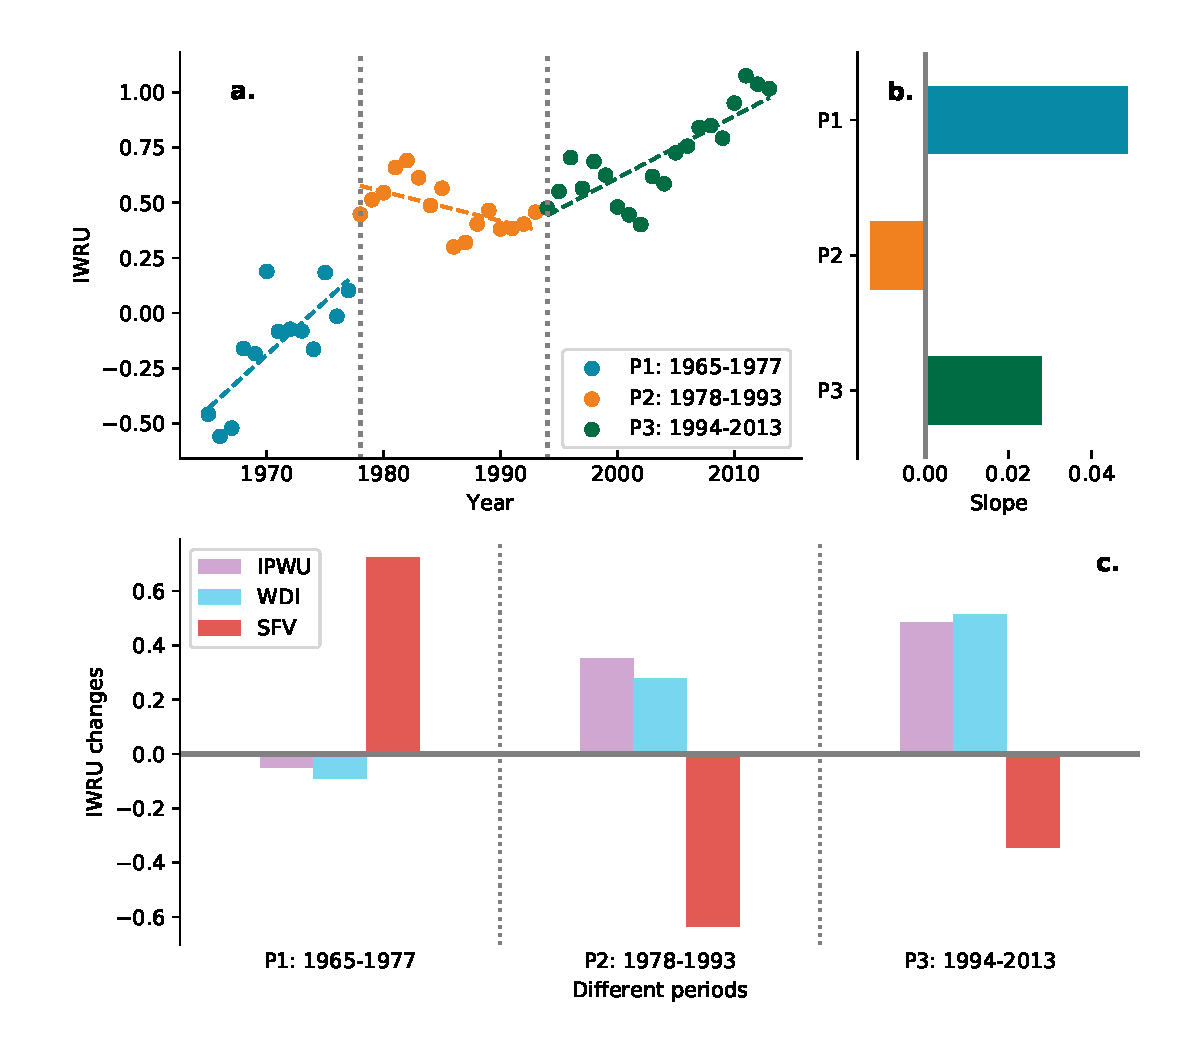
\includegraphics[width=\linewidth]{../../figures/main_text/index.pdf}
	\caption{Changes of the IWRU index. 
	\textbf{A,} with two change points in 1978 and 1994, three periods were detected in trend of the IWRU.
	\textbf{B,} changes of IWRU in three periods have various slopes, while the second period have a negative growths rate.
	\textbf{C,} changes of the IWRU within three certain periods, which have different main contributors.
	}
	\label{fig:IWRU}
\end{figure}
% 接下来分句介绍每个阶段的特征
% 第一阶段
In the first period (P1, 1965-1978), the IWRU index had a rapidly increasing 
and the lightening of water stresses made the most striking contribution (124\%), 
while tendentiousness and pattern of the water utilization had slight negative contribution.
% 第二阶段
In the second period (P2, 1979-1994), the IWRU index experienced a slight drop, 
despite positive contributions of tendentiousness and pattern of water utilization,
because of increasing stresses on water resource playing a larger negative role (-146\%). 
% 第三阶段
However, as the further increasing of positive contributions of water utilization tendentiousness and pattern, 
and decelerations of water stresses in the third period (P3, 1995-2013), a positive growth of the IWRU returned.
% 总而言之,每个阶段都由水资源利用的不同维度提供最大的正向作用
As a result, each period is various in the most striking positive contributors to IWRU, 
corresponding to different dimensions of water utilization.

% 用水三个维度的组合呈现出阶段特征明显
Combining the three dimensions of water resources utilization, further more, 
sub-index regard to different water utilization dimensions were aggregative distinguishably in each same period, 
whose regimes show clear phase-characteristics (Figure~\ref{fig:phases}).
\begin{figure}%[htbp]
	\centering
	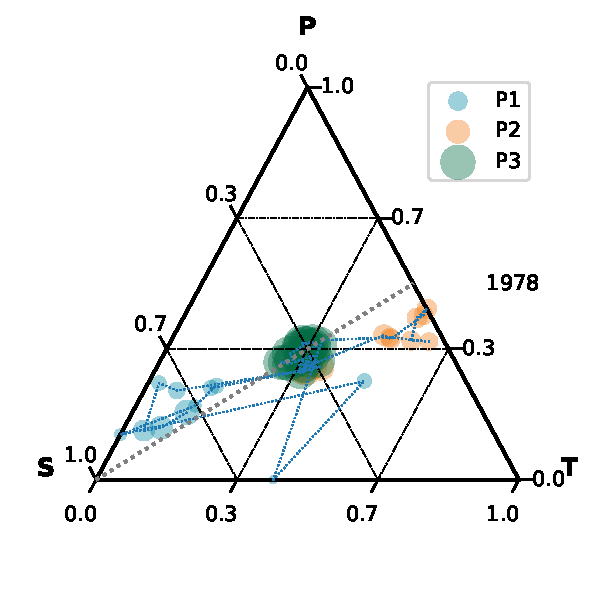
\includegraphics[width=\linewidth]{../../figures/main_text/phases.pdf}
	\caption{Combination of three dimensions (S: stresses; T: tendentiousness; P: pattern) in different periods. 
	Size of the points denoting values of the IWRU: the mean of the P1 phase is 0.10, while 0.14, 0.19 in P2 and P3.
	The red indicator line in this ternary plot denotes 1:1 contributions between tendentiousness (T) and patterns (P).
	Two key change points (1978, 1994), along with the beginning (1965) and the ending (2013) of research period, are labelled.}
	\label{fig:phases}
\end{figure}
% 第一阶段到第二阶段
At the very beginning of research period (1965), high water stress domain the regime, 
while it experienced a large shift after entering P2 since 1978, 
with a change in the proportion of contributions between tendentiousness and pattern, too.
% 第三阶段集中
In contrast, the three dimensions' contribution were similar from 1994 into P3 to 2013, 
making the points highly concentrated at the centre of the ternary diagram for that period.
% 总之,出现制度
Taken all together, the three phases delineate distinct water resource utilization regimes, 
corresponding each period of.

%tag 结果2
\subsection*{Changes of water utilization between regimes}
% 在不同的维度下各阶段进行对比,可以发现不同的水资源利用体系间存在明显差异。
A comparison of the phases under different dimensions reveals notable differences regarding water utilization
between each water use regime (Figure~\ref{fig:dimensions}).
\begin{figure*}%[htbp]
	\centering
	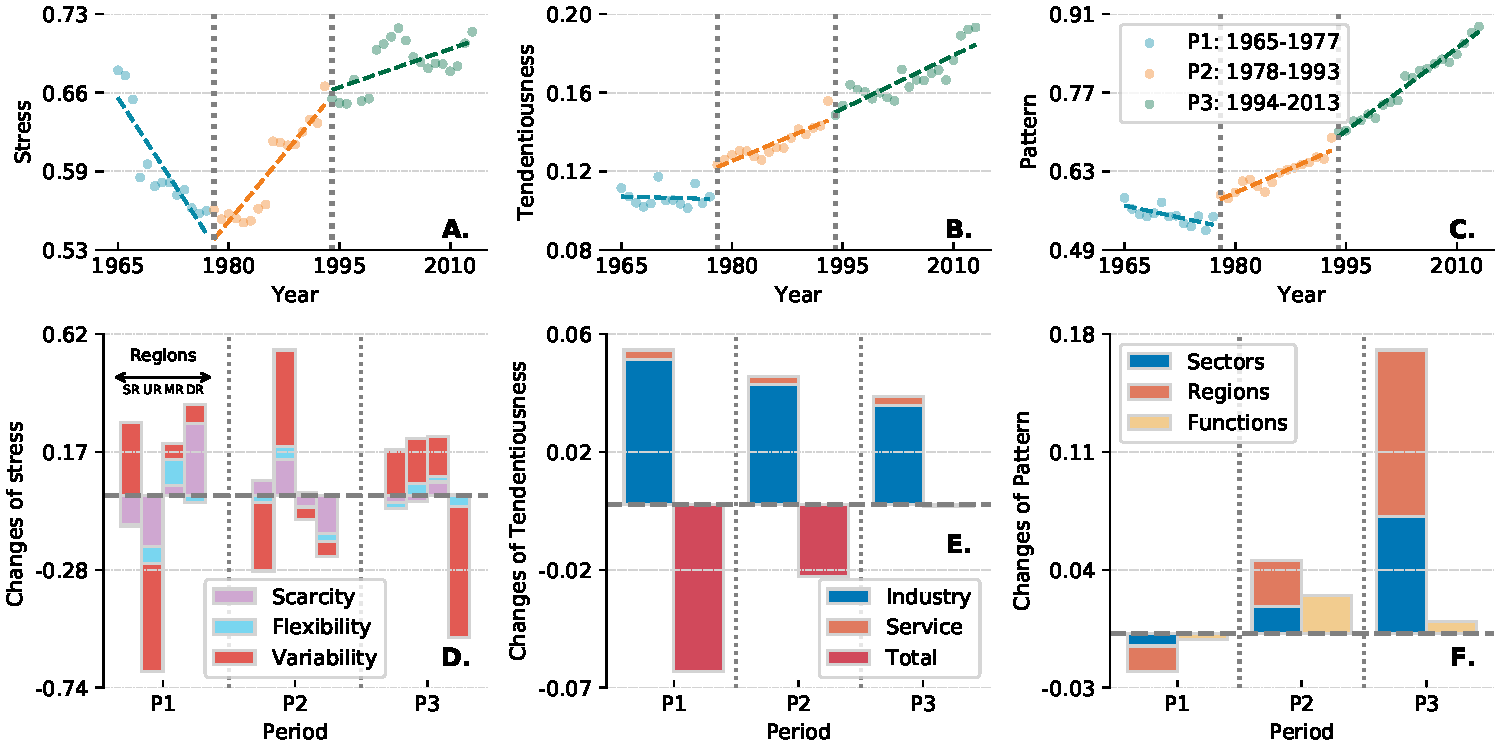
\includegraphics[width=\linewidth]{../../figures/main_text/dimensions.pdf}
	\caption{
		Changes in different dimensions of water resources utilization regime.
		\textbf{A,} changes of scarcity-flexibility-variability water stresses index (SFV-index).
		\textbf{B,} changes of non-provisioning water share, indicating water utilization tendentiousness.
		\textbf{C,} changes of water utilization pattern index.
		}
	\label{fig:dimensions}
\end{figure*}
% 从阶段一到阶段二,水资源压力的变化最为明显
Moving from the regime in P1 to P2, the most striking change is the reversal of the trend in water stresses (Figure~\ref{fig:dimensions}A).
% 由于水资源压力由稀缺性、灵活性和变异性共同决定,P1-P2的变化主要看SFV
The P1, when water resources were the most abundant period, also had the least water consumption, 
while most of which were flexible water utilization.
Despite the rapid rise in water use during that period, numerous reservoirs were also built during this period, 
which increased storage capacities in each water-demand region to relief water resource stresses (SI).
However, entering P2, although water consumptions continued to increase, 
the number of new reservoirs was significantly reduced and the total storage capacity of each region was hardly increasing any more. 
Coupled with declining natural water resources, the water stress index of the basin was rapidly increasing.
% 另一方面,P2-P3,持续变化的水资源利用倾向与格局
On the other hand, as the most positive contributors to the IWRU index in P2 and P3, separately, 
tendentiousness and patterns of water utilization were still enlarging their impacts (Figure~\ref{fig:dimensions}B and C). 
% 首先是用水比例的变化
Representing tendentiousness of water utilization, 
increasing non-provisioning share of water utilization were mainly contributed by larger industrial water consumptions and minor total water uses, 
while the influence of both is waning.
% 再讨论用水格局的变化
However, patterns of water utilization, with accelerating changes and larger contributions to the IWRU, 
were mainly benefited from the convergence of development paces between regions and the basin-wide intersectoral water balance.
% 最后,每个阶段起
In summary, the changes in various aspects of the water use characteristics of the Yellow River Basin over the past 60 years 
are reflected in the changes in the corresponding indicators of the three dimensions.

% tag 结果3
\subsection*{Causes of water utilization regime changes}

\begin{figure}%[htbp]
	\centering
	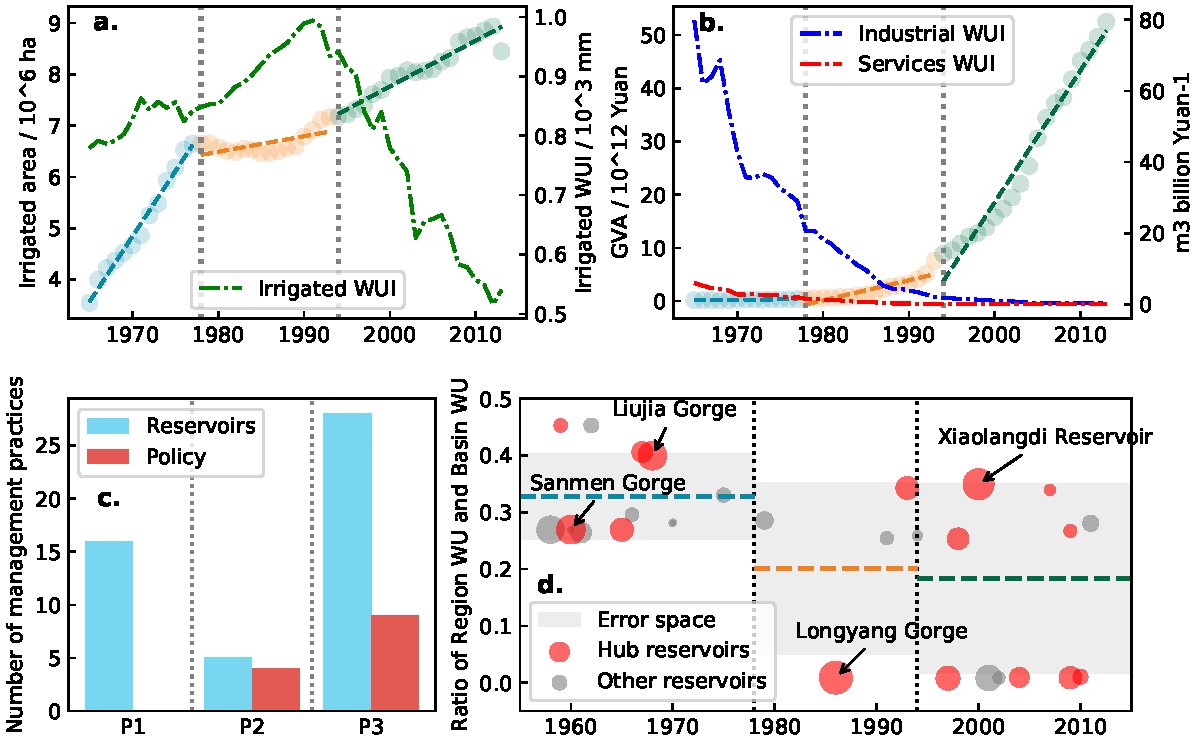
\includegraphics[width=\linewidth]{../../figures/main_text/causes.pdf}
	\caption{
		Causes of water utilization regime shifts: economy growths, efficiency changes, and managements.
		\textbf{A.} Total irrigated area and water consumption per unit of irrigated area.
		\textbf{B.} Gross values added of industry and services, and their water use density (WUI) respectively.
		\textbf{C.} Number of management practices in different periods, including policy and reservoirs.
		\textbf{D.} Constructions' finished time of each new reservoir and their located regions' water use percentages in basin's total water use, at that time. Red ones denote hub reservoirs in the basin, which plays a role in integrated water management. Size of the points indicates their magnitude of water storage capacities. Some important or special reservoirs' name are denoted: (1) Xiaolangdi reservoir and Three Gorge Reservoir were constructed mainly responsible for managing sediments of the Yellow River. (2) Liujia Gorge, Longyang Gorge, were constructed mainly responsible for managing water flood discharge and storage. Therefore, these marked reservoirs are significant for the entire basin, far crucial than regional development.
	}
	\label{fig:Causes}
\end{figure}

Some main drivers caused the changes of water utilization regime (Figure\ref{fig:Causes}).
% 经济总量提升导致资源耗竭的加速。
(1) The expansion of irrigated area and the economic growth of industry and services are key to the
changes in the tendentiousness of water utilization in P1 and P2.
During P1, irrigated agricultural area in the Yellow River basin expanded rapidly at a rate of xx/year, 
and agriculture was the dominant water use (xx \% of the total).
After entering P2, however, while the expansion of irrigated area stalled, 
industry and services gradually took off, which took up more water resources.
% 用水关系的变化
(2) Efficiency of water use sparkly changed during the P3.
Although both industrial services output and irrigated agricultural area resumed expansion in P3, 
both their output per unit and water consumption per unit area experienced significant declines.
As a result, after the P3, the proportions of the different water-using sectors tend to average out 
while the total water consumption remains stable.
% 不断变化的管理模式。
(3) Changing water management practice contributed between different periods.
In P1, most of the reservoirs are built in regions where water use is growing, 
and the trend of growth in storage capacity and growth in water demand remain relatively consistent regionally.
In P2, on the other hand, the number of additional reservoirs decreases significantly. 
Within P3, the number of reservoirs increases significantly again, 
but the growth of storage capacity does not match the growth of water demand.

% tag 讨论
\section*{Discussion}

\subsection*{Transition Framework}
% 普遍存在的稳态转换可以由渐变或突变造成,而人类压力在世界范围内都是稳态转换最重要的驱动因素之一。
Widespread regime shift of coupled systems can be caused by gradual or abrupt changes, 
where anthropogenic stresses are among the most important drivers of. 
% 而随着人类干预的加深,水循环出现了自然-社会二元结构,主导当前人水系统的互馈过程。
With the accumulation of human interventions, 
a natural-social binary structure of the water cycle has emerged, 
dominating the current feedbacks of the human-water systems.
% 我们的研究结果表明,与社会-生态系统的过渡过程类似,水资源利用体系的变化也存在类似稳态转换的阶段性特征,并最终呈现出自然-社会二元结构。
According to our results, 
regime shifts as transitional phases of water utilization regimes, 
similar to evolution of social-ecological system, 
is one of the most important characteristics towards natural-social binary structure.
% 因此,我们在总结黄河流域变化过程的基础上,进一步概念化了水资源利用制度的过渡框架。
As such, we summarized a transition framework of the water utilization regimes, which conceptualizes a general trajectory towards a natural-social binary water cycle.

\begin{figure*}%[htbp]
	\centering
	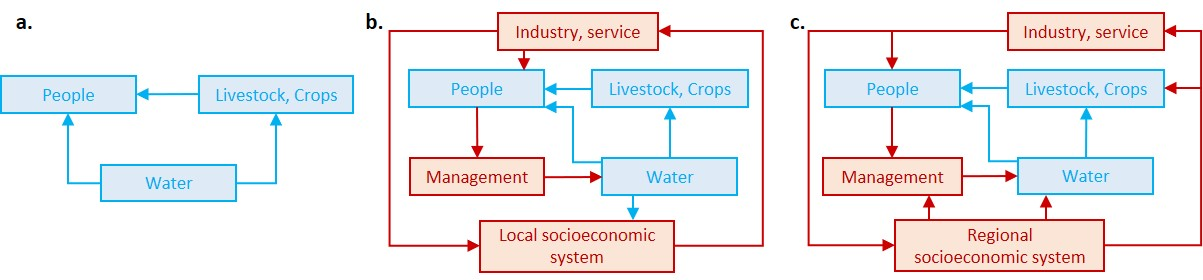
\includegraphics[width=\linewidth]{../../figures/main_text/framework}
	\caption{
		Transition framework of the water utilization regime towards natural-social binary cycle.
		\textbf{A. Natural cycle:} As a kind of direct provisioning resource, the main functions of water resource is to support crop, livestocks and human-beings, which are the basic ecological services.
		\textbf{B. Local binary cycle:} With local socio-economic systems developing, industry and services (also known as the secondary and the tertiary industry) calling for further water consumptions.
		However, as their ecological services generated through the socio-economic cycle, water resources play a non-provisioning role. What's more, better organized socio-economic system and developed technology gives humans the will and ability to better manage water resources and change since this phase, with intensive intervention in the natural water cycle. 
		\textbf{C. Basin binary cycle:} Entering this phase, with further developing in more economically efficient industries and services, trade-off between whose water demands with provisional water demands becomes prominent. Rather than determined by local socio-economic systems, water withdrawals and management act as considerations within the entire basin more, therefore. 
	}
	\label{fig:framework}
\end{figure*}


% 在水循环向二元系统过渡过程中,存在几个明显的特征。
Towards natural-social binary cycle, there are two obvious features between different transition phases  (figure \ref{fig:framework}).
% 水资源利用制度包括压力、倾向性、格局三个重要因素,三个指标在过渡框架中随着不断变化。
Throughout the above transition phases towards binary water cycle, 
three dimensions of water utilization regime are various, following three laws of evolution respectively.
Firstly, although stresses on water resources increases by economic expansion boosting water demands, 
socio-economic progress responding to resource scarcity because of better management and increased water use efficiency. 
For Example...
Secondly, the non-provisioning part of water demands further growths and 
tendentiousness of water utilization continually changes, 
as humans are more dependent on benefits from non-provisioning part of water supply.
Thirdly, With closer socio-economic ties between regions and between regions and river basins, 
the geographic scope of resource supply and demand allocation is expanding, 
leading to changing patterns of water utilization.
By combining the three dimensions, water utilization regimes have a tendency of transitional evolution.


% 综上所述,社会对水资源的利用模式作为一个人-水互馈系统,存在阶段性过渡特征。
For the Yellow River Basin, 
In addition to the Yellow River Basin, which is the focus of this study, 
human-water relations in major river basins around the world 
can be explained by the phases of the transitional framework.
For examples, \dots \dots.
In summary, our proposed transitional framework for the nature-society binary water cycle is general in nature.

\subsection*{Development Traps}
% 不同的流域位于过渡的不同阶段,面临的问题也存在区别,主要包括资源陷阱和结构陷阱两类。
Since each basin at different transition phase, 
they are facing different development traps regarding water utilization, 
leading an unsustainable trajectory. 
Like social-ecological systems and other complex systems, 
coupled human-water system disintegrate may occurred under the gradual pressure of rising resources, 
or collapse emerged because of structural mismatches.
A number of studies have identified transformation as an important way out of unsustainable trajectory, 
and different types of transformation are required according to dominating phases and traps of systems.
Thus, it is crucial to distinguish major development traps 
based on the transition framework of water utilization regimes.


% 世界各大流域面临的问题。资源开发早期容易陷入资源陷阱;流域发展后期容易陷入结构陷阱。
According to case studies from watersheds around the world, 
big river basins often face a resource trap at the beginning of their development, 
while highly developed ones often face a structural trap.
% 黄河流域的发展过程,资源开发P2阶段陷入了资源陷阱(表现形式 xxx)。
For the Yellow River Basin, 
after the successive expansion of agriculture and industrial services during the P1 and P2 phases, 
the utilization rate of surface water resources has reached 80\% of the natural runoff, 
far exceeding the internationally recognized threshold of 40\%.
Although water management measures in P1 (construction of numerous reservoirs) 
mitigated the pressure on water resources due to accelerated development, 
the pressure on water resources rebounded rapidly during P2, 
when the number of new reservoirs declined significantly.
These have led to increasingly severe outages and groundwater depletion of the Yellow River from P2 onwards, 
and the Yellow River basin had been in a notable resource trap.
% 资源困局可能普遍存在
In any case, the xxx and xxx basins have a development history similar to that of the Yellow River, 
suggesting that resource distress may be widespread in the early stages of the transition.


% 后来摆脱了资源陷阱(表现形式 xxx)。
Faced with a clear resource trap, a clear transformation path towards integrated basin management was proposed
that has contributed to the gradual escape of the Yellow River from the resource trap.
.....
In short, these integrated management practices made the utilization of water resources into a regime of unified scheduling, 
in the Yellow River Basin 
to escape from the “resource trap” of economic expansion and accelerated resource depletion.
Similarly, 
many of the world's major river basins have eventually moved towards a system of integrated management and integrated dispatch, 
especially the XXX and XXX basins, 
where water resources are extremely scarce.


% 展望:未来还可能陷入结构陷阱,(表现形式:用水效率悖论的同时,灵活性进一步降低,
However, Despite achieving integrated management and escaping through increased water efficiency, 
basins still face new structural traps and require further transformation.
Firstly, in line with paradox of irrigation efficiency \ref{graftonParadoxIrrigationEfficiency2018}, 
significant improvement in agricultural irrigation efficiency (or decline in water use intensity) 
has been accompanied by a resurgence in irrigated area, 
resulting in an unabated and weak upward trend in water stress.
% 水资源压力仍在增大,而节水能力已经进入瓶颈,倾向性贡献减少)
As integrated basin allocation dominates water allocation, 
the propensity to allocate water between non-supply industries, such as industrial services, 
and agriculture is becoming fixed.
At the same time, the flexibility of water use is declining since domestic water use and thermal water use growth rapidly. 
Typically, similar to other cases, these may lead to a reduction in watershed resilience 
and leave highly coupled human-water systems facing greater vulnerability to collapse 
-- a typically structural trap.
% 下一步:可以通过统一调控,调整格局来调整结构,突破结构陷阱。
% 总结:整个流域需进一步转型与适应,以实现高质量发展。
Therefore, based on the identification of the current basin transition stage and development dilemma, 
further transitional governance is still needed to achieve high-quality sustainable development of the basin.




%tag 研究方法
\matmethods{Please describe your materials and methods here. This can be more than one paragraph, and may contain subsections and equations as required. Authors should include a statement in the methods section describing how readers will be able to access the data in the paper. 
	
	\subsection*{Water utilization regime index}
	Example text for subsection.
	\subsubsection*{Stresses}
% 提出了很多的指标度量水压力,如水资源压力指数,水资源xxx等
	Various metrics, therefore, proposed for water stress 
	(e.g. water scarcity, water stresses index, scarcity-flexibility-variability index), 
	where the dimensions of human impact are increasingly valued.
	% 其中SFV指数比较有用
	Among of them, by taking changes of water flexibility and variability into account, 
	the scarcity-flexibility-variability (SFV) index focus more on dynamic responses to water resources in developing perspective,
	which considered a valid indicator of temporal changes in water stresses.
	\subsubsection*{Lopsidedness}
	% xxx等人通过考虑消费品中的水消耗提出了虚拟水理论
	% 但随着水资源利用方式的变迁,在其基础上兴起的水足迹研究,则进一步泛化了水相关的产品和服务概念。
	% 如今,世界非产品形式供给于人类的水资源已达xx%,范围包含了xxxxxx等方式,人类在“消耗水”向“利用水”和的倾斜。

	\subsubsection*{Patterns}

	\subsection*{Change points detection}
	
	\subsection*{Contribution decomposition}
}

\showmatmethods{} % Display the Materials and Methods section

\acknow{Please include your acknowledgments here, set in a single paragraph. Please do not include any acknowledgments in the Supporting Information, or anywhere else in the manuscript.}

\showacknow{} % Display the acknowledgments section

% Bibliography
\bibliography{my-papers}
	
\end{document}